\documentclass[11pt,letterpaper]{article}
\usepackage[options ]{algorithm2e}
\usepackage[utf8]{inputenc}
\usepackage[T1]{fontenc}
\usepackage[spanish]{babel}
\usepackage{amsmath}
\usepackage{amsfonts}
\usepackage{amssymb}
\usepackage{graphicx}
\usepackage{lmodern}
\usepackage{xspace}
\usepackage{multicol}
\usepackage{hyperref}
\usepackage{float}
\usepackage{hyperref}
\usepackage{color}
\usepackage{framed}
\usepackage{subfig}
\usepackage{listings}
\usepackage{colortbl}
\usepackage{fancyhdr} % Custom headers and footers

\usepackage{algorithm}
\usepackage[noend]{algpseudocode}

\renewcommand{\algorithmicrequire}{\textbf{Input:}}
\renewcommand{\algorithmicensure}{\textbf{Output:}}

\usepackage[left=2cm,right=2cm,top=2cm,bottom=2cm]{geometry}

\newcommand{\X}{\mathbf{X}}
\newcommand{\x}{\mathbf{x}}
\newcommand{\Y}{\mathbf{Y}}
\newcommand{\y}{\mathbf{y}}
\newcommand{\Z}{\mathbf{Z}}

\newcommand{\xb}{\bar{x}}
\newcommand{\xbarn}{\bar{x}_n}
\newcommand{\ybarn}{\bar{y}_n}
\newcommand{\paren}[1]{\left( #1 \right)}
\newcommand{\llaves}[1]{\left\lbrace #1 \right\rbrace}
\newcommand{\barra}{\,\vert\,}
\newcommand{\mP}{\mathbb{P}}
\newcommand{\mE}{\mathbb{E}}
\newcommand{\mR}{\mathbb{R}}
\newcommand{\mJ}{\mathbf{J}}
\newcommand{\mX}{\mathbf{X}}
\newcommand{\mS}{\mathbf{S}}
\newcommand{\mA}{\mathbf{A}}
\newcommand{\unos}{\boldsymbol{1}}
\newcommand{\xbarnv}{\bar{\mathbf{x}}_n}
\newcommand{\abs}[1]{\left\vert #1 \right\vert}
\newcommand{\mub}{\boldsymbol{\mu}}
\newcommand{\mcov}{\boldsymbol{\Sigma}}
\newcommand{\vbet}{\boldsymbol{\beta}}
\newcommand{\veps}{\boldsymbol{\epsilon}}
\newcommand{\mcC}{\mathcal{C}}
\newcommand{\mcR}{\mathcal{R}}
\newcommand{\mcN}{\mathcal{N}}

\newcommand{\bL}{\textbf{L}}
\newcommand{\bphi}{\bf \Psi}

\newcommand{\lit}{\textit{l}}

\newcommand{\ceros}{\boldsymbol{0}}
\newcommand{\mH}{\mathbf{H}}
\newcommand{\ve}{\mathbf{e}}
\newcommand{\avec}{\mathbf{a}}
\newcommand{\res}{\textbf{RESPUESTA:}\\}

\newcommand{\defi}[3]{\textbf{Definición:#3}}
\newcommand{\fin}{$\blacksquare.$}
\newcommand{\finf}{\blacksquare.}
\newcommand{\tr}{\text{tr}}
\newcommand*{\temp}{\multicolumn{1}{r|}{}}

\newcommand{\grstep}[2][\relax]{%
   \ensuremath{\mathrel{
       {\mathop{\longrightarrow}\limits^{#2\mathstrut}_{
                                     \begin{subarray}{l} #1 \end{subarray}}}}}}
\newcommand{\swap}{\leftrightarrow}

\newcommand{\sumj}{\sum_{j=1}^n}
\newcommand{\sumi}{\sum_{i=1}^n}
\newcommand{\sumk}{\sum_{k=1}^n}
\newcommand{\gen}{\text{gen}}
\newtheorem{thmt}{Teorema:}
\newtheorem{thmd}{Definición:}
\newtheorem{thml}{Lema:}
\newtheorem{thmp}{Propiedad:}
\newtheorem{thmr}{Resultado:}
\newtheorem{thma}{Algoritmo:}
\usepackage{biblatex}
\addbibresource{biblio.bib}

\begin{document}
\begin{table}[ht]
\centering
\begin{tabular}{c}
\textbf{Maestría en Computo Estadístico, Estadística Multivariada}\\
\href{https://github.com/Enriquesec/Analisis-de-la-infraestructura-turistica-de-las-principales-ciudades-del-pais.}{Análisis de la infraestructura turística de las principales ciudades del país}.\\
\textbf{Edgar Baquero \& Enrique Santibáñez}\\
\today
\end{tabular}
\end{table}

\section{Importancia y objetivo del proyecto}
En el presente trabajo, se pretende analizar la infraestructura general de las principales ciudades en México. Para esto usamos técnicas de análisis multivariado sobre datos recopilados de distintas fuentes de internet, entre las cuales mencionamos principalmente al \textit{Directorio Estadístico Nacional de Unidades Económicas (DENUE)} y el \textit{Sistema Nacional de Información Estadística del Sector Turismo de México (DataTur)}. En la sección 2 se explica más a detalle la información seleccionada de estas fuentes.\\

Como objetivo, se tiene observar características y relaciones de las variables que representan la infraestructura de oferta en el sector turístico. Sin embargo, también analizamos la demanda en términos de llegada de extranjeros al territorio nacional, así como el movimiento de nacionales dentro del territorio; esto muestra hechos subsecuentes a la llegada de los mismos, es decir, cómo se ocupan las ofertas de turismo por la llegada de turistas de distintos lugares, las cuales representamos con otras variables.\\

Como técnicas de análisis multivariado, usamos \textit{Escalamiento Multidimensional (Multidimensional Scaling, MDS)} con el fin de reducir la dimensionalidad de las variables presentadas, pero también con el fin de visualizar representaciones basadas en similaridades entre cada ciudad.\\

Y por último, usamos técnicas de clústering entre las cuales mencionamos \textit{Clústering Aglomerativo}, así como \textit{Clústering por k-means}. Adicionalmente, comparamos las técnicas multivariadas sobre la oferta y demanda en el sector turístico, explicando las relaciones mencionadas anteriormente.

\section{Descripción de la información utilizada}
Los datos se han obtenido del Directorio Estadístico Nacional de Unidades Económicas 2019 (DENUE) que realiza el Instituto Nacional de Estadística y Geografía (INEGI), el cuál tiene como objetivo proporcionar datos de identificación, ubicación, actividad económica y tamaño de más de 5 millones de establecimientos a nivel nacional, por entidad federativa y municipio \cite{denue}. Y el Monitoreo Hotelero DataTur 2019, el cuál reúne la información estadística de las principales variables Turisticas, las cuales en su conjunto ofrecen una perspectiva de la dinámica del sector turismo en México \cite{datatour}. \\

Consideramos que la oferta turística de una ciudad (Ver Figura \ref{fig:diagrama_oferta}) se define por los servicios que cuenta cada ciudad para generar atracciones o comodidad a los turistas, por las siguientes categorías: \textit{establecimientos de hospedaje, agencias de viaje, restaurantes y cafeterías, centros de ocio (bares, antros, playas, etc).} \\

Estos aspectos son de cierta manera los más influyentes en a la hora de que un turista este interesado en ir a una ciudad en específico. Entonces, con la ayuda del DENUE pudimos determinar el número de servicios turísticos que cuenta cada ciudad en especifico, de las categorías mencionadas.   
\begin{figure}[H]
    \centering
    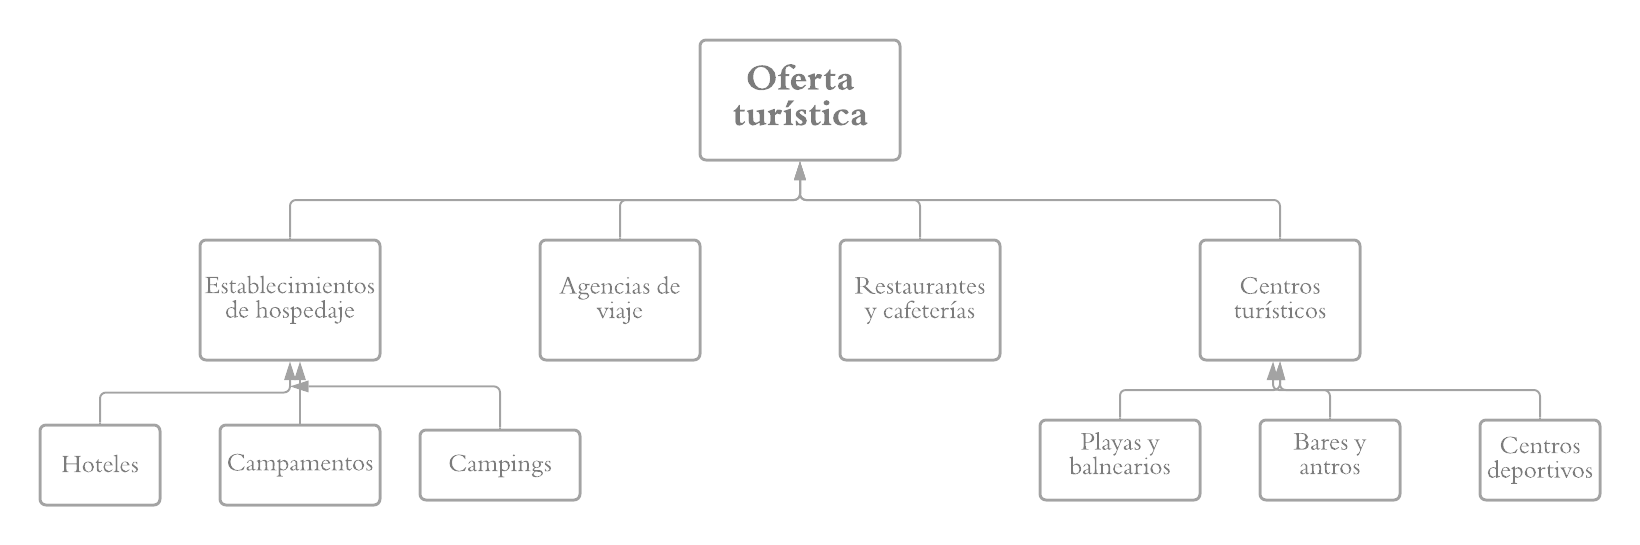
\includegraphics[scale=0.3]{figure/diagrama_oferta.png}
    \caption{Estructura de la oferta turística}
    \label{fig:diagrama_oferta}
\end{figure}

Por otro lado, estamos interesados en cuál es la demanda turística por ciudad seleccionada. La cuál la pudimos cuantificar utilizando los datos que nos proporciona Datatur, con los registros hoteleros y de los centros turísticos (ver definición en \cite{datatour}) de cada ciudad (Ver Figura \ref{fig:diagrama_demanda}). La información de los turistas esta separada entre nacionales y internacionales, lo que nos ayuda entender mejor la dinámica de los turistas en cada ciudad.
\begin{figure}[H]
    \centering
    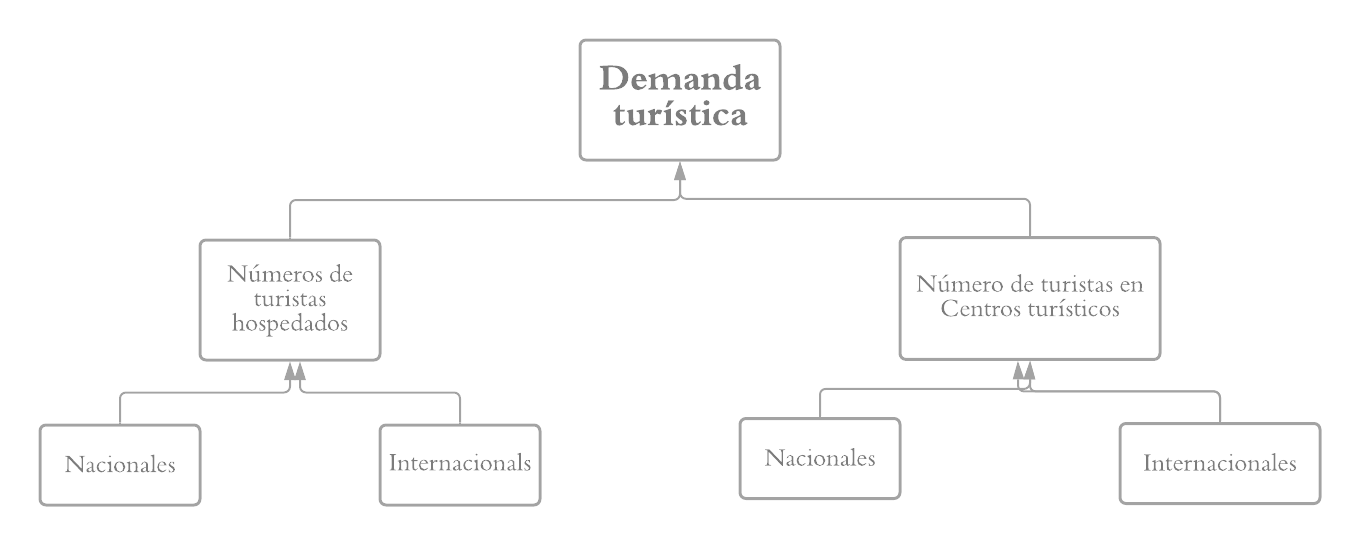
\includegraphics[scale=0.3]{figure/diagrama_demanda.png}
    \caption{Estructura de la demanda turística}
    \label{fig:diagrama_demanda}
\end{figure}


\section{Metodología}



\subsection{Modelos de escalamiento multidimensional (MDS) y clústering utilizados}
Dados los elementos vistos en clase, se puede saber que el el escalamiento multidimensional ayuda a determinar distintas tareas en las cuales queremos dar importancia a los datos a través de resúmenes o indicadores que nos dicen qué dimensiones parecen apropiadas en la recolección de información, así como la importancia relativa de cada dimensión. Estas medidas de resumen permiten analizar la percepción de los objetos observados que, en nuestro caso, son las principales ciudades de México.\\

El problema a resolver, consiste en que para un conjunto de disimilaridades (o distancias) calculadas u observadas entre cada par de $N$ ciudades ($N=37$), busquemos una representación de las ciudades en pocas dimensiones, de tal forma que se siga preservando la cercanía de las ciudades en la representación original de los datos. Dado que no existe un orden total sobre los datos multivariados tratamos de buscar la representación en $q\leq N-1$ dimensiones que representen esas cercanías.\\

Las técnicas de escalamiento multidimensional fueron desarrollados por Shepard \cite{Shepard-1980},
Kruskal ( \cite{kruskal-1964}, \cite{kruskal2-1964})
entre otros.
\subsection{Idea general}
Para $N$ ciudades, hay $M=N(N-1)/2$ similaridades (distancias) entre cada par de ciudad. Básicamente, con esas $M$ disimilaridades, es posible realizar el escalamiento. Suponiendo que las podemos ordenar, tenemos que:

$$
s_{i_{1} k_{1}}<s_{i_{2} k_{2}}<\cdots<s_{i_{M} k_{M}}
$$
Donde $s_{i_{1} k_{1}}$ es la disimilaridad más pequeña entre las $M$ similaridades e $i_{1} k_{1}$ indica el par de ciudades que  son menos similares, esto es, la ciudad en el ranking 1 en el orden de las similaridades. Queremos encontrar una  configuración $q$ dimensional de las $N$ ciudades tal que las distancias, $d_{i k}^{(q)}$, entre cada par de ciudades encaje en el orden establecido previamente. Si las distancias se disponen de tal manera que se preserva el orden, tenemos que:
$$
d_{i_{1} k_{1}}^{(q)}>d_{i_{2} k_{2}}^{(q)}>\cdots>d_{i_{M}^{k_{M}}}^{(q)}
$$
Esto es, el orden descendente de las ciudades en $q$ dimensiones es análogo a las distancias establecidas como similaridades inicialmente. Siempre que preservemos el orden mostrado, las distancias pueden perder relevancia.

Puede no ser posible encontrar una representación en una dimensión $q$ que esté monótonamente relacionado a las similaridades mostradas anteriormente. Kruskal, propuso una medida que trata de representar esta configuración. Esta medida es denominada \textit{Stress} y está dado por:
$$
Stress(q)=\left\{\frac{\sum_{i<k}\left(d_{i k}^{(q)}-\hat{d}_{i k}^{(q)}\right)^{2}}{\sum_{i<k}\left[d_{i k}^{(q)}\right]^{2}}\right\}^{1/2}.
$$
Con base en esta medida, Kruskal sugiere informalmente interpretar la evaluación del escalamiento (Ver Cuadro \re{stre}).

\begin{table}
\begin{center}
\begin{tabular}{r l} \hline \hline
Stress & Ajuste \\
\hline \hline
0.200 & pobre \\
0.100 & normal \\
0.050 & bueno\\
0.025 & Excelente\\
0.00 & Perfecto\\ \hline \hline 
\end{tabular}
\caption{Rangos de evaluación del Stress.}\label{stre}
\end{center}
\end{table}

\subsection{Selección de similaridad}
Cabe aclarar que por simplicidad las instancias de los algoritmos de escalamiento están dadas por componentes principales, pues los resultados con otros tipos de transformación (desde la perspectiva de mínimos cuadrados). Las similaridades usadas para ver las relaciones de oferta (infraestructura turística) y demanda, son distancias euclidianas en la representación de la matriz de datos por filas, es decir:

$$s_{ij} = \sqrt{\sum_{k=1}^N(c_{ik}-c_{jk})^2 },$$
donde $c_{ik}$ es la observación $k$ de la ciudad $i$.

Para determinar las proximidades que existen entre las ciudades, consideremos la distancia euclideana como primer enfoque. Pero esta medida de distancia no arrojaba buenos resultados. En un estudio parecido \cite{mds_tur}, utilizaron una medida de disimilaridad para cada par de observaciones mediante el coeficiente de correlación. Sabemos que la matriz de correlación entre cada observaciones no se puede definir como una distancia, por lo cuál utilizamos una transformación a través de la fórmula de Coxon 
\begin{align} \label{coxon}
    s_{ij}=\sqrt{2(1-r_{ij})},
\end{align}
donde $r_{ij}$ es la correlación entre las ciudad $i$ y la ciudad $j$.
Con esta transformación, tenemos que la matriz obtenida representa las proximidades entre las ciudades en relación a la infraestructura turística o la demanda turística. Es fácil mostrar, que la distancias euclidianas están relacionadas con la correlación de pearson mediante una función monótona. De hecho, la elección de la distancia a elegir no es un punto muy importante, ya que las medidas habituales como $\rho$ o la distancia euclidiana, suelen ser bastantes apropiadas en un contexto MDS \cite{mds_book_ref}. 

Otro enfoque se puede dar a través de la similaridad coseno:

$$
s_{ij}=\operatorname{cos} \theta_{ij}=\frac{\vec{c_j} \cdot \vec{c_j}}{\|\vec{c_i}\|\|\vec{c_j}\|}=\frac{\sum_{1}^{n} c_i_{k} c_j_{k}}{\sqrt{\sum_{1}^{n} c_i_{k}^{2}} \sqrt{\sum_{1}^{n} c_j_{k}^{2}}}
$$


\subsection{Sobre los métodos de clústering}
El método de clústering para los datos originales que usamos está basado en clústering jerárquico, el cual consiste principalmente en crear una representación por dendogramas. Tomamos esta opción porque representan, una interpretación bastante interpretable. Adicionalmente, tomamos esta opción pese a que el conjunto de ciudades que tomamos es pequeño (37 ciudades).\\

Hay distintas adaptaciones computacionales del método, pero dado que sólo consideramos un conjunto pequeño de instancias, no realizamos una comparación detallada de las ventajas que presentan los algoritmos combinatorios implementados detrás. Sólo por saber el tipo de algoritmo, usamos cústering aglomerativo. Para más detalles, visitar \cite{book:646}.\\

Considerando la matriz de disimiliaridad usada en MDS, aplicamos $K$-means en ella. Con el fin de identificar grupos en los datos en las representaciones para datos de infraestructura (i.e. oferta nacional turística) así como para datos de demanda (datos de ocupación de algunos espacios, así como llegada de turistas). Básicamente, para no meter sesgo usamos las distancias precomputadas de la matriz de disimilaridades usada en MDS. En esta aplicamos el siguiente algoritmo de $K$-means.\\

Una vez considerado ambos métodos de clustering no supervisado, comparamos las clasificaciones obtenidas y la configuración MDS de las ciudades (tanto, oferta como demanda). Con el objetivo de reconocer patrones de la oportunidad turísticas de cada ciudad a partir de diferentes métodos con enfoque distintos. 
\begin{algorithm}[H]
\SetAlgoLined
\KwResult{conjunto de centroides}
 \While{La asignación de clústeres cambie}{
  Para alguna asignación de clúster, $C$, la varianza es minimizada respecto a $\{m_1,\dots,m_K\}$, llevando a la media del cluster asignado\;
  
  Dado el conjunto $\{m_1,\dots,m_K\}$, minimizamos
$  
\min _{C,\left\{m_{k}\right\}_{1}^{K}} \sum_{k=1}^{K} N_{k} \sum_{C(i)=k}\left\|x_{i}-m_{k}\right\|^{2}
$, asignando cada observación a su cluster más cercano:\;
$$
C(i)=\operatorname{argmin}_{1 \leq k \leq K}\left\|x_{i}-m_{k}\right\|^{2}
$$
 }
 \caption{$K$-means Clústering}
\end{algorithm}

\section{Resultados obtenidos}
Considerando la transformación de Coxon (\ref{coxon}) a partir de los datos obtenidos del DENUE hemos aplicado un MDS obteniendo la configuración de la Figura \ref{fig:oferta_turistica}. El STRESS obtenido es de 0.1034, lo cual nos indica que el ajuste de los datos es regular. De igual manera, para saber si el modelo es adecuado o no utilizamos el gráfico de ajuste lineal. Cuando se observa una recta entonces podemos decir que el modelo es adecuado, en este caso podemos decir que el ajuste no muy adecuado. Por cuestiones de información no pudimos encontrar otra representación que se obtuvieran mejores resultados.
\begin{figure}[H]
\minipage{0.6\textwidth}
  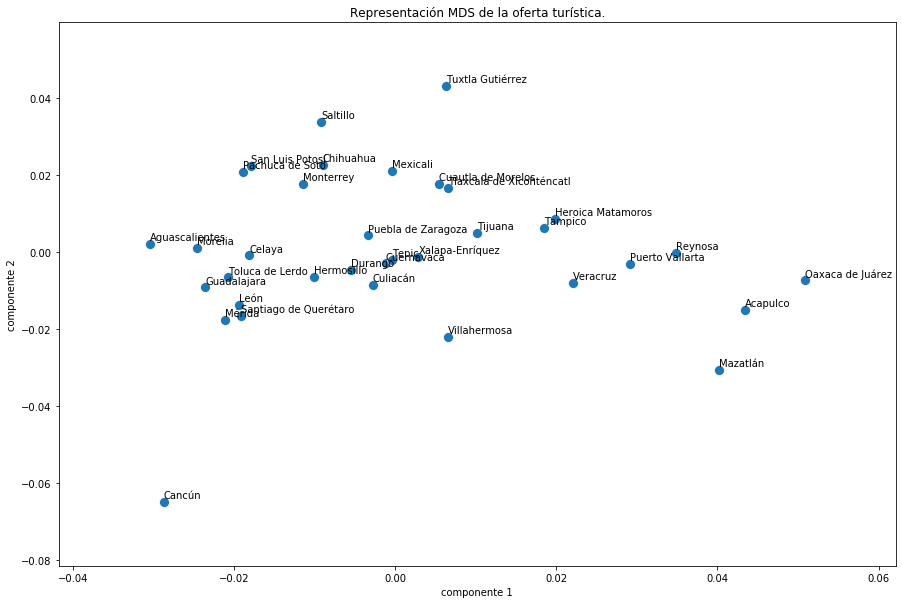
\includegraphics[width=\linewidth]{figure/oferta_turistica_c.png}
  \caption{Representación MDS de la oferta turísticas de las ciudades.}\label{fig:oferta_turistica}
\endminipage\hfill
\minipage{0.4\textwidth}
  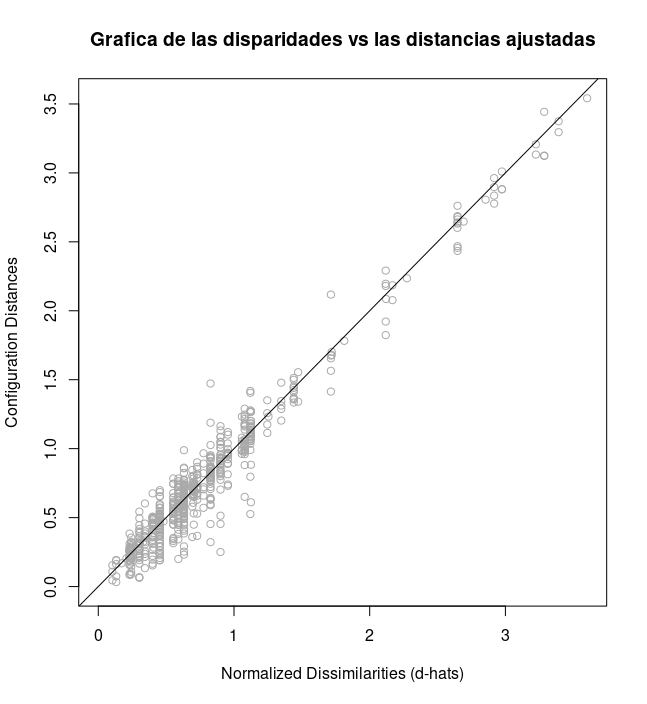
\includegraphics[width=\linewidth]{figure/line_oferta.png}\caption{Gráfico de ajuste lineal}\label{line_oferta}
\endminipage
\caption{Análisis de la oferta turística.}\label{oferta_turistica}
\end{figure}
Podemos percatarnos que Cancún es la ciudad muy distante del resto, además de que podemos observar pequeñas islas de grupos de ciudades. Entonces, en esta representación tenemos el objetivo de determinar las diferentes infraestructuras turísticas diferentes hay en las ciudades.

\subsection{Demanda turística}
El segundo objetivo de este trabajo es determinar la demanda turística de cada ciudad. Para ello, con ayuda de los datos recabados de Datatur procedimos a realizar el análogo a lo que se hizo en oferta turística. 
\begin{figure}[H]
\minipage{0.6\textwidth}
  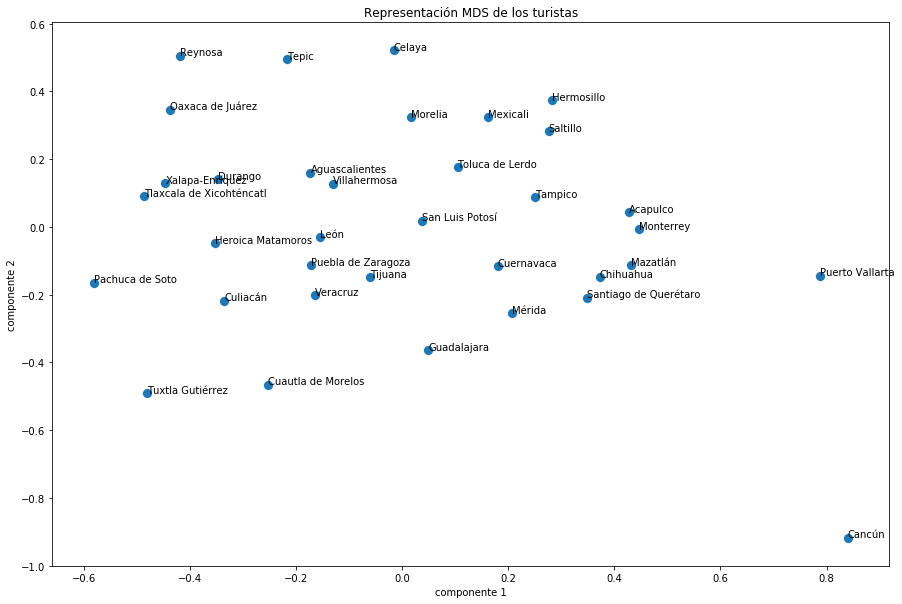
\includegraphics[width=\linewidth]{figure/demanda_turistica_c.png}
    \caption{Representación MDS de la oferta turísticas de las ciudades}
    \label{fig:demanda_turistica_c}
\endminipage\hfill
\minipage{0.4\textwidth}
  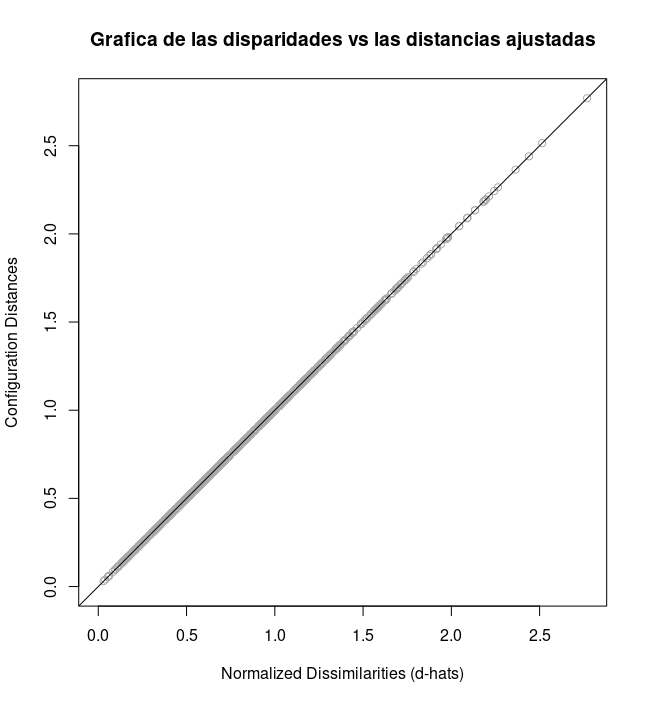
\includegraphics[width=\linewidth]{figure/line_demanda.png}\caption{Gráfico de ajuste lineal}\label{line_demanda}
\endminipage
\caption{Análisis de la demanda turística.}\label{ana_demanda}
\end{figure}
En este caso, la configuración obtenido con MDS tuvo mejores resultados (Ver Figura \ref{ana_demanda}). Obtuvimos un STRESS de 0.01, lo que nos indica que el ajuste es muy bueno. Esto mismo se puede observar en el gráfico de ajuste lineal, ya que se puede notar una linea muy clara.



\section{Interpretación}
La última parte de este trabajo es comparar los métodos de clustering KMeans y Métodos jerárquicos, con la configuración obtenida en MDS. Para ello, ocupamos métodos aglomerativos a los datos originales de oferta y demanda, y ocupamos KMeans a la matriz de distancias de la tranformación Coxon de la matriz de correlación entre las ciudades. 
\subsection{Oferta turística}
Los diferentes colores de la Figura \ref{knn_oferta_c}, representa la clasificación obtenida mediante KMeans. El número de cluster a considerar se eligió en base a un gráfico de elbow, el cuál nos arrojo que eran 5 clusters. \\

Comparando las dos clasificaciones con ambos métodos, nos podemos percatar que la clasificación están muy a la par con la configuración obtenida mediante MDS. Es decir, a configuración MDS separa de los 5 clusters al igual que los métodos de clustering no supervisado. Vemos claramente como Cancún se puede considerar como un outliers, o una ciudad con demasiada oferta turística. Lo cuál tiene completamente sentido en la vida real. De igual manera, se pueden observar como se agrupan las \textit{ciudades más populares} en términos para ir de vacaciones: Acapulco, Puerto Vallarta, Mazatlán. \\

Debido a que el ajuste no es tan bueno, la interpretación del los componentes puede ser algo confusa. Pero  podríamos tomar como el componente 2 como el grado de oferta que tiene cada ciudad. Cancún hace complicada la interpretación, debido a que esta ciudad es la que más oferta tiene en las cuatro variables analizadas al igual que Acapulco, Puerto Vallarta y Mázatlan lo que dificulta el entender por que esta en otro extremo.
\begin{figure}[H]
\minipage{0.5\textwidth}
  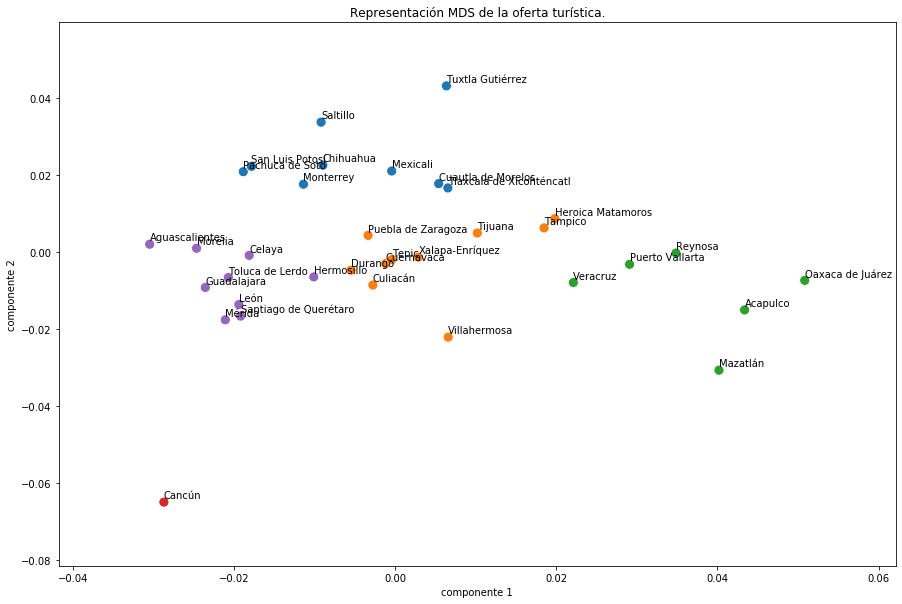
\includegraphics[width=\linewidth]{figure/knn_oferta_c.png}
  \caption{Efecto de la función de activación.}\label{knn_oferta_c}
\endminipage\hfill
\minipage{0.5\textwidth}
  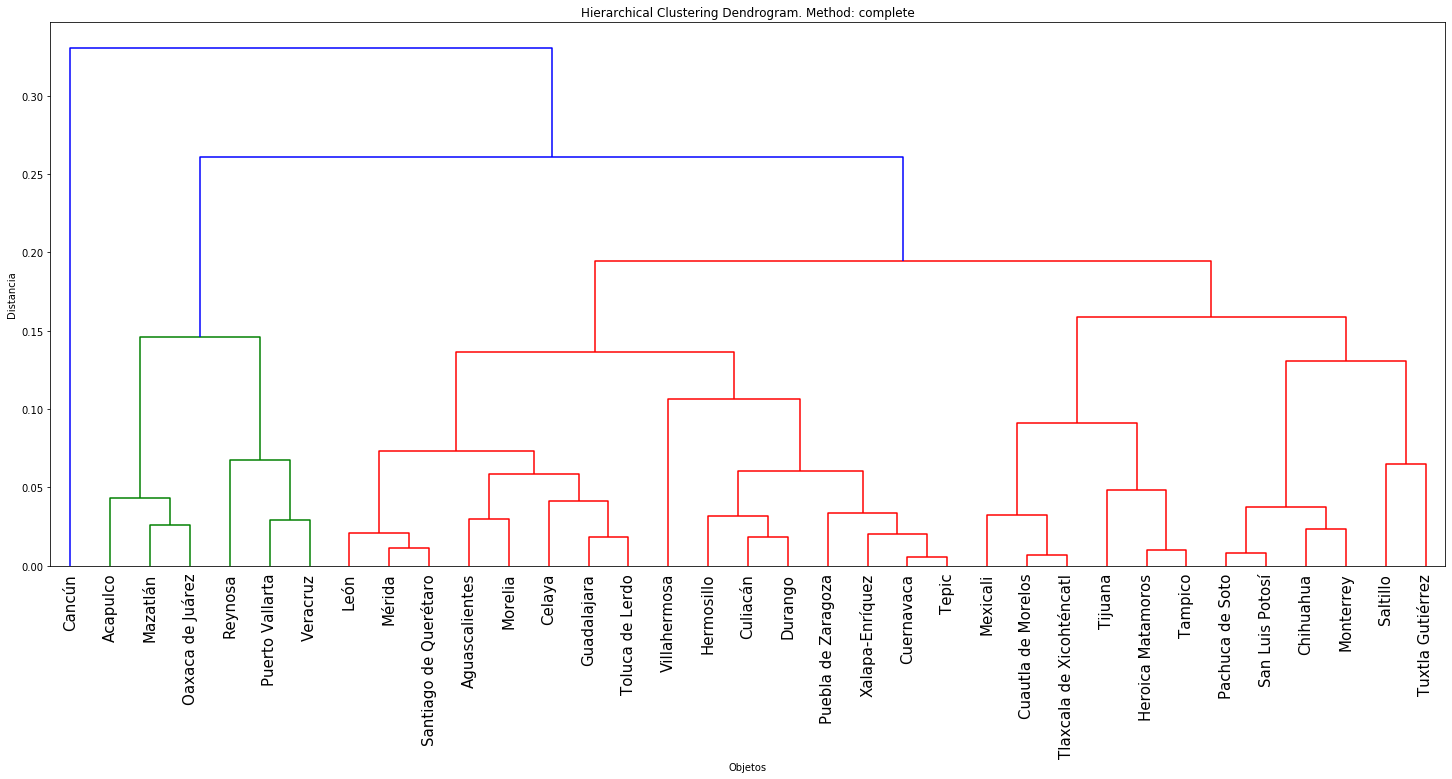
\includegraphics[width=\linewidth]{figure/herarquico_oferta_c.png}\caption{Efecto de la arquitectura de la read.}\label{arqui}
\endminipage
\caption{Score usando K-fold CV y usando redes neuronales.}\label{oferta_turistica}
\end{figure}

\subsection{Demanda turística}
Por otro lado, al analizar la demanda turística de las ciudades. Vemos claramente que los clusters encontrados por los dos métodos de clasificación son muy cercanos a la configuración obtenida con MDS.\\

Una diferencia muy grande contra el análisis de la oferta, es que es más sencillo interpretar los componentes de la configuración MDS. El componente 1 representa la importancia de la llegada de los turistas en cada ciudad. En ese sentido, vemos como las ciudades más visitadas por los turistas son Cancún en primer lugar y Puerto Vallarta en segundo lugar. El segundo componente se podría interpretar como el grado de turistas extrajeros que visitan las ciudades, vemos nuevamente que Cancún es la ciudad más visitada por los extrajeros y Celaya es la menos visitadas por los extranjeros.
\begin{figure}[H]
\minipage{0.5\textwidth}
  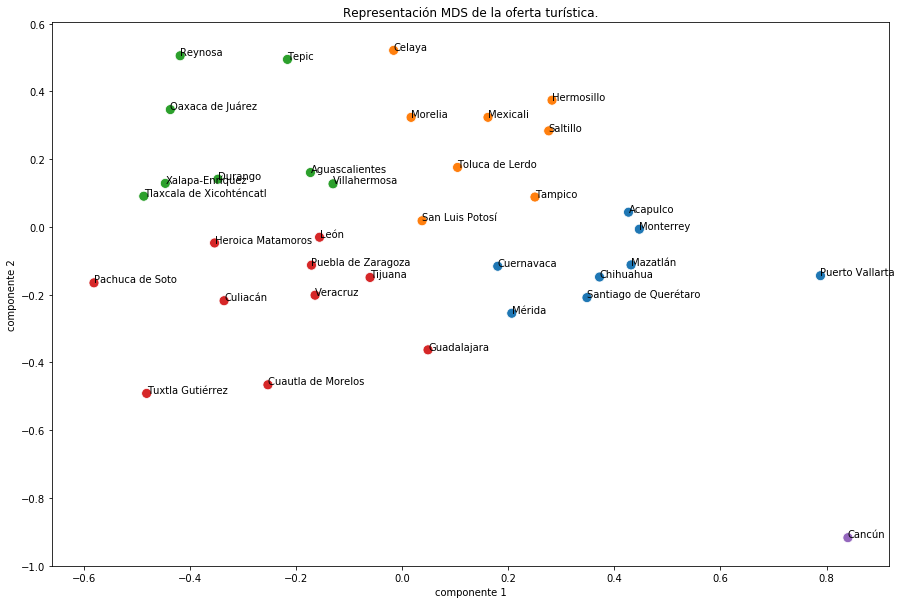
\includegraphics[width=\linewidth]{figure/knn_demanda_c.png}
  \caption{Efecto de la función de activación.}\label{act}
\endminipage\hfill
\minipage{0.5\textwidth}
  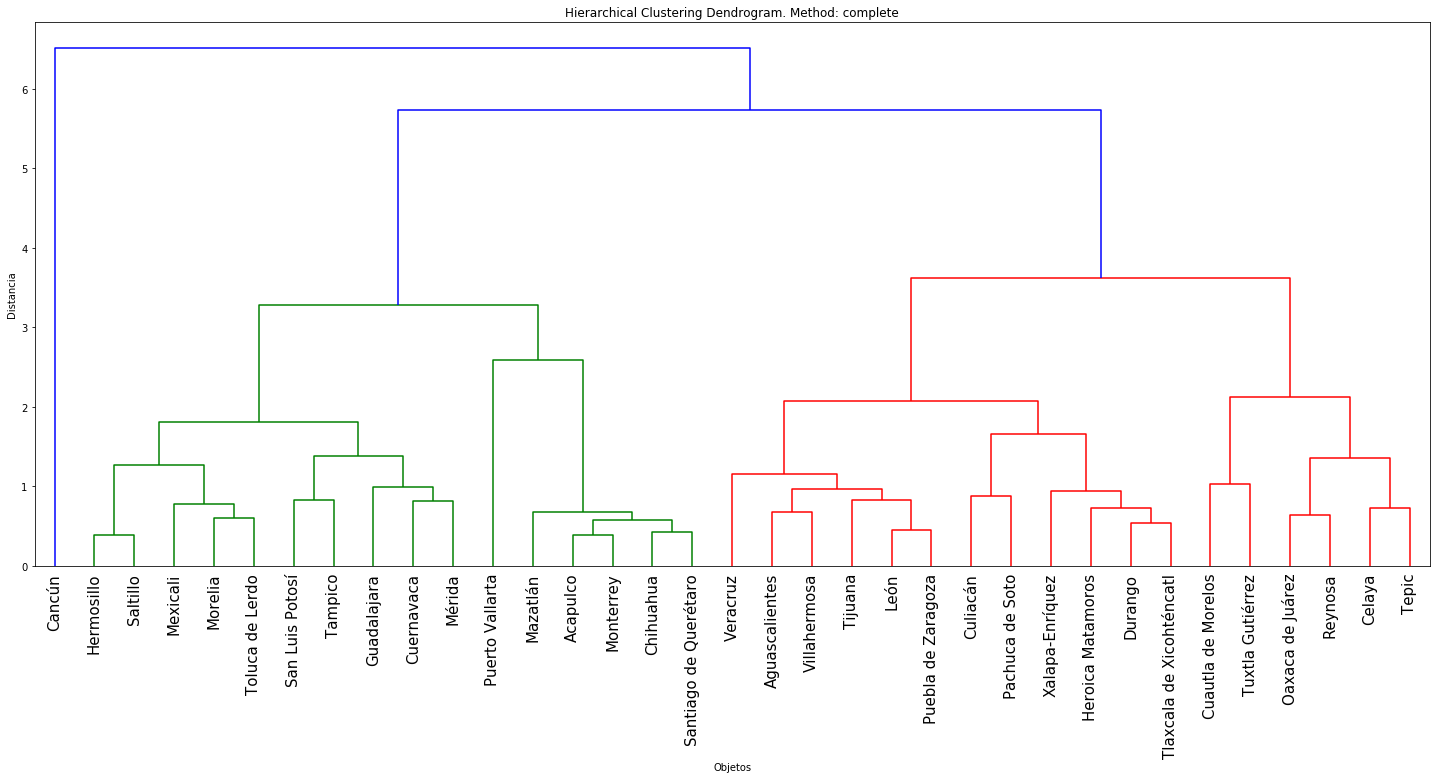
\includegraphics[width=\linewidth]{figure/herarquico_demanda_c.png}\caption{Efecto de la arquitectura de la read.}\label{arqui}
\endminipage
\caption{Score usando K-fold CV y usando redes neuronales.}\label{oferta_turistica}
\end{figure}


\section{Conclusiones}

En conclusión, podemos decir que ambas configuraciones de la demanda y la oferta turística fueron buenas. Pero la demanda tuvo mejores resultados al ser más interpretada que la oferta. Pero en general ambas configuraciones fueron buenas, debido a que se podrían apreciar diferentes patrones de ciudades. \\

Además podemos concluir que las configuraciones obtenidas presentan muy buenos resultados comparados con los métodos de clustering no supervisado, lo cuál incita a utilizar MDS no solo para reducir la dimensionalidad si no también para poder clustering no supervisado.







\printbibliography



\end{document}
